\documentclass[a4paper,11pt,oneside]{article}

% To use this template, you have to have a halfway complete LaTeX
% installation and you have to run pdflatex, followed by bibtex,
% following by one-two more pdflatex runs.
%
% Note thad usimg a spel chequer (e.g. ispell, aspell) is generolz
% a very guud ideo.

\usepackage[utf8]{inputenc}
\usepackage[a4paper,top=3cm,bottom=3cm,left=3cm,right=3cm]{geometry}
\renewcommand{\familydefault}{\sfdefault}
\usepackage{helvet}
\usepackage[T2A, T1]{fontenc} %%T2A is needed to support russian
\usepackage[russian, english]{babel}     %% typographie française
\usepackage{csquotes}
\usepackage[style=numeric,language=english]{biblatex}
\usepackage{parskip}		%% blank lines between paragraphs, no indent
\usepackage[margin=1cm]{caption}%% give long captions a margin
\usepackage{booktabs}           %% typesetting nice tables
\usepackage[outputdir=build]{minted}%% typesetting code nicely
\usepackage[pdftex]{graphicx}	%% include graphics, preferrably pdf
\usepackage[pdftex]{hyperref}	%% many PDF options can be set here
\pdfadjustspacing=1		%% force LaTeX-like character spacing

\newcommand{\mylastname}{Stupnikov}
\newcommand{\myfirstname}{Aleksandr}
\newcommand{\mynumber}{00101010}
\newcommand{\myname}{\myfirstname{} \mylastname{}}
\newcommand{\mytitle}{Context-Aware Remote Procedure Calls in Kotlin}
\newcommand{\mysupervisor}{Prof.~V.~Confused}

%% My commands
\newcommand{\term}[1]{\textit{#1}}
\newcommand{\makedefinition}[3][]{\textbf{#2}\ifthenelse{\equal{#1}{}}{}{~(#1)}~--- #3.}
\newcommand{\kotlini}[1]{\mintinline{kotlin}{#1}}
\newcommand{\ki}[1]{\kotlini{#1}}

\hypersetup{
  pdfauthor = {\myname},
  pdftitle = {\mytitle},
  pdfkeywords = {},
  colorlinks = {true},
  linkcolor = {blue}
}

\addbibresource{msc-sample.bib}

\begin{document}
\pagenumbering{roman}

\thispagestyle{empty}

\begin{flushright}
  
\includegraphics[scale=0.8]{msc-logo}
\end{flushright}
\vspace*{40mm}
\begin{center}
  \huge
  \textbf{\mytitle}
\end{center}
\vspace*{4mm}
\begin{center}
  \Large by
\end{center}
\vspace*{4mm}
\begin{center}
  \LARGE
  \textbf{\myname}
\end{center}
\vspace*{20mm}
\begin{center}
  \Large
  Master Thesis in Computer Science and Software Engineering
\end{center}
\vfill
\begin{flushleft}
  \large
  Submission: \today \hfill Supervisor: \mysupervisor \\
  \rule{\textwidth}{1pt}
\end{flushleft}
\begin{center}
  Constructor University $|$ Constructor Institute of Technology
\end{center}

\newpage
\thispagestyle{empty}

\begin{center}
  \Large \textbf{Statutory Declaration}
  \vspace*{8mm}
\end{center}

\begin{center}
  \begin{tabular}{|l|p{85mm}|}
    \hline
    Family Name, Given/First Name & \mylastname, \myfirstname \\
    Matriculation number & \mynumber \\
    Kind of thesis submitted & Master Thesis \\
    \hline
  \end{tabular}
  \vspace*{8mm}
\end{center}

\subsection*{English: Declaration of Authorship}

I hereby declare that the thesis submitted was created and written
solely by myself without any external support. Any sources, direct
or indirect, are marked as such. I am aware of the fact that the
contents of the thesis in digital form may be revised with regard to
usage of unauthorized aid as well as whether the whole or parts of
it may be identified as plagiarism. I do agree my work to be entered
into a database for it to be compared with existing sources, where
it will remain in order to enable further comparisons with future
theses. This does not grant any rights of reproduction and usage,
however.

This document was neither presented to any other examination board
nor has it been published.

\subsection*{German: Erklärung der Autorenschaft (Urheberschaft)}

Ich erkläre hiermit, dass die vorliegende Arbeit ohne fremde Hilfe
ausschließlich von mir erstellt und geschrieben worden ist. Jedwede
verwendeten Quellen, direkter oder indirekter Art, sind als solche
kenntlich gemacht worden. Mir ist die Tatsache bewusst, dass der
Inhalt der Thesis in digitaler Form geprüft werden kann im Hinblick
darauf, ob es sich ganz oder in Teilen um ein Plagiat handelt. Ich
bin damit einverstanden, dass meine Arbeit in einer Datenbank
eingegeben werden kann, um mit bereits bestehenden Quellen
verglichen zu werden und dort auch verbleibt, um mit zukünftigen
Arbeiten verglichen werden zu können. Dies berechtigt jedoch nicht
zur Verwendung oder Vervielfältigung.

Diese Arbeit wurde noch keiner anderen Prüfungsbehörde vorgelegt
noch wurde sie bisher veröffentlicht.

\vspace{20mm}

\dotfill\\
Date, Signature

\newpage

\section*{Abstract}

Consider this a separate document, although it is submitted together
with the rest. The abstract aims at another audience than the rest
of the proposal. It is directed at the final decision maker or
generalist, who typically is not an expert at all in your field, but
more a manager kind of person. Thus, don't go into any technical
description in the abstract, but use it to motivate the work and to
highlight the importance of your project.

(target size: 15-20 lines)

A large subset of modern software uses network interactions extensively. One of the languages that
is actively used to develop such software is Kotlin. However, standard for Kotlin technologies like
REST for organizing network interactions are overly explicit and require writing a lot of
additional code by applying specific patterns. Such code is usually called \term{boilerplate code}.

In this thesis, an alternative mechanism for organizing network interactions in Kotlin is
proposed. This mechanism uses approach less common for Kotlin, called Remote Procedure Call (RPC).
This approach allows the invocation of Kotlin function on a remote machine, provided the function
is annotated in a special way. Such annotated functions are called \term{remote functions}.

The novelty of the mechanism proposed in this work lies in the usage of implicit parameters: information
required from the call-site context. In contrast with traditional RPC, proposed approach uses
context in which remote function is invoked to determine on what machine function should be
executed. This leads to more implicit organization of network interactions and as a result greatly
reduces boilerplate code required for network heavy applications.

\newpage
\tableofcontents

\clearpage
\pagenumbering{arabic}

\section{Introduction}

This, like the rest, addresses fellow experts from your field (but
not from your particular topic of research). Here you should
technically connect to the main concepts from that field and give an
outline of your project, stating the research/engineering question
that you want to get answered by your project.

(target size: 1-2 pages)

Nowadays, Kotlin programming language is used frequently for developing software that relies
heavily on network interactions. Such software includes distributed networks, microservices,
client-server applications and much more. Usually code base of all such applications can be roughly
separated into two parts: part responsible for actual business logic and part responsible for
network interactions. While the former part differs significantly from program to program, network
interactions part is usually very similar for a wide variety of applications. This leads to the
abundance of boilerplate code in the said part. For convenience from now on we will call part of
the program source code responsible for network interactions \term{network part} of the program. It
is desired to make network part of the program as small and simple as possible, because this would
allow developers to think less about network and concentrate on the actual business logic.

However, standard ways to implement network part in Kotlin are not well suited for making this part
concise. The problem lies in the excessive explicitness of the standard approaches. For example,
REST architecture frequently used in Kotlin forces developers to manually write routing logic as
well as part of the serialization and deserialization logic. This has its benefits because it
provides fine control over the network part logic, but often this fine-tuning capabilities is not
needed. Frameworks like gRPC and kRPC are a step further from REST in attempt to decrease
boilerplate. But their usage still requires describing and creating RPC services explicitly,
arbitrary functions cannot be executed remotely. Other popular approaches like one used in Retrofit
framework are basically variations of the named approaches.

The goal of the thesis is to develop alternative approach to organizing network interactions in
Kotlin that will make network part smaller and easier by reducing amount of boilerplate code.

To achieve this goal we took a look at RPC in Kotlin from another perspective not common for
object-oriented languages. The problem with existing RPC frameworks for Kotlin is their focus on
RPC services, special classes which code is generated during compile time using method signatures
from user defined interface. Even though this approach is the only option for strict OOP languages
(like Java) it can be improved for Kotlin which is not purely OOP language. In this paper we
explore using coeffects, a concept from the world of functional programming, to implement RPC
framework that require to write much less boilerplate code than more traditional RPC frameworks.
More than that, this approach makes network code easily distinguishable from the rest of the
program. In Kotlin programming with coeffects can be expressed by using experimental language
feature called \term{context parameters}, which allows function has several receiver parameters, 
that implicitly passed to the function from the invocation context.

\textbf{This work has the following structure:}
\begin{enumerate}
  \item Section 2 reviews background and related work on organizing network interaction both in Kotlin ecosystem and outside that.
  \item Section 3 describes architecture of the developed approach.
  \item Section 4 evaluates the approach by using small applications and comparing them with standard approaches.
  \item Section 5 concludes, discuss limitations and future work.
\end{enumerate}

\section{Background and Related work}

This part should make clear which question, exactly, you are
pursuing, and why your project is relevant/interesting. This is the
place to explain the background and to review the existing
literature. Where does your project extend the state of the art?
What weaknesses in known approaches do you hope to overcome? If you
have carried out preliminary experiments, describe them here.

(target size: 5-10 pages)

This section will give an overview of RPC as whole, as well as specific frameworks used in Kotlin ecosystem
to implement RPC. Also concepts used in this thesis, like coeffects and Kotlin context parameters, will
be explained here.

Proposed approach is a specific version of RPC, because of that it makes sense to only compare it
to other RPC approaches that are used in Kotlin. The most popular ones are gRPC and new Kotlin RPC.
We solve problem that RPC frameworks require to write boilerplate code, because they require to
declare services. Only methods of these services can be executed remotely, but methods of normal
classes and top level functions cannot. Basically all the existing RPC frameworks for Kotlin use 
Remote Method Invocation (RMI), the object-oriented programming analog of RPC, even though Kotlin is
not entirely OOP language.

Information in callable map is enough to generate public API of the service.

\subsection{RPC}

Even though the concept of RPC is well known in the community, it is still better to provide some
understanding of RPC that is used in this work.

\makedefinition[RPC]{Remote procedure calls}{a communication protocol which allows an application
executing functions on a remote machine (commonly using a shared computer network) as if these 
functions were executed on the machine where the application is running}

\makedefinition{Remote function}{function that can be executed on a remote machine}

The goal of RPC is to hide details of network communication from an application and make remote 
functions calls look like ordinary function calls. This paradigm allows programmer to think less about
network details and more about core logic of the application. 

The idea of RPC is not new and dates back 1970s \cite{white_high-level_1976} with enterprise 
implementations appearing roughly in the 1980s \cite{birrell_implementing_1984}.

\subsection{Distributed Objects}

RPC does not translate well in object-oriented world, where interactions between objects residing
on different machines are required. That is why when object-oriented languages became popular
specific form of RPC was developed. This form is called \term{RMI}, and it is a way to build
communication between \term{distributed objects} \cite{wollrath_distributed_1996} \cite{tanenbaum_distributed_2006}.

\makedefinition{Distributed Objects}{objects that can be accessed from remote machines}

\makedefinition[remote method invocation]{RMI}{communication protocol which allows an application
executing methods of distributed objects on a remote machine}

Classic forms of RMI in their fullness are not popular nowadays. Implementations like Java RMI or 
CORBA are not used in a modern production code. Modern approaches try to be more lightweight and explicit
they do not try to hide network interactions completely from the developer \cite{ryan_grpc_2015}

\subsection{gRPC}

\cite{noauthor_grpc_nodate}

\subsection{Kotlin RPC}

\subsection{Coeffects}

\subsection{Kotlin Ecosystem}
In the framework developed as part of this thesis many technologies from Kotlin Ecosystem are used.
Therefore, it makes sense to quickly introduce this technologies.

\subsubsection{Kotlin Coroutines}

\subsubsection{kotlinx.serialization}

\subsubsection{Ktor}

\subsubsection{Kotlin context parameters}


\section{Kotlin Remote Implementation}

This is the technical core of the thesis. Here you lay out your how
you answered your research question, you specify your design of
experiments or simulations, point out difficulties that you
encountered, etc.

(target size: 5-10 pages)

Framework that was developed in thesis is called \term{Kotlin Remote}. And from now on we will refer 
to that this way. 

\subsection{Remote functions}

Function that can be executed on remote machine (aka remote functions) are the integral part of any 
RPC framework.

In order to reason about remote functions two terms should be introduced: client and server.
In RPC world \term{client} is machine from which remote call is made and \term{server}
is target machine of this remote call, machine where call is actually executed.

\subsubsection{Client} \label{client-section}

Let us take a look at how remote call is done on the client in Kotlin Remote. In order to call
a function on a remote machine it is necessary to pass to this function some information specific
to remote call, including address of the target machine and a way to serialize function arguments
and deserialize its result. In existing RPC frameworks this information is provided to the function
using stub. To better understand what stub is and how it provides necessary information for remote
call, let us take a look at the example for Kotlin RPC in the figure \ref{krpc_remote_call}. User
have to create instance of \kotlini{KtorRpcClient}, which is configured with remote host URL
and serialization schema. Then using this client user can create service stub
\kotlini{client.withService<PizzaShop>()}, where \kotlini{PizzaShop} is interface which
implementation is generated automatically by Kotlin RPC. Such an interface is usually called \term{service}
which remote machine provides.

\begin{figure}[!h]
  \begin{minted}{kotlin}
  @Rpc
  interface PizzaShop { suspend fun orderPizza(pizza: Pizza): Receipt }
  fun main() = runBlocking {
    val client: KtorRpcClient = HttpClient { ... }.rpc {
      url { host = "localhost" }
      serialization { json() }
    }

    val pizzaShop: PizzaShop = client.withService<PizzaShop>()

    pizzaShop.orderPizza(Pizza("Pepperoni"))
  }
  \end{minted}
  \caption{Remote function call in Kotlin RPC}\label{krpc_remote_call}
\end{figure}

Stub \kotlini{pizzaShop} use client with which stub was created to make remote calls.
It has some drawbacks:
\begin{enumerate}
  \item Top level functions can not be called using this approach
  \item User have to declare interface just for remote functions
  \item When calling methods of the stub user does not know that calls results in network 
  interaction, it is completely implicit
  \item When user wants to call remote functions of the same service on several target machines, several
  stubs have to be created 
\end{enumerate}

gRPC uses virtually the same approach as Kotlin RPC but a bit more cumbersome.

But stubs is not the only way to provide remote function with information it needs. Alternative
approach is used in functional programming. Let us take a look at remote calls in RPC framework for
Haskell programming language named Servant \cite{noauthor_servant_nodate}.

\begin{figure}[!h]
  \begin{minted}{haskell}
  position :: Int -> Int -> ClientM Position
  hello :: Maybe String -> ClientM HelloMessage

  queries :: ClientM (Position, HelloMessage)
  queries = do
    pos <- position 10 10
    message <- hello (Just "servant")
    return (pos, message)

  run :: IO ()
  run = do
    Right (pos, message) <- runClientM queries ... "localhost"
    print pos
    print message
  \end{minted}
  \caption{Remote function call in Servant}\label{servant_remote_call}
\end{figure}

Here \mintinline{haskell}{position} and \mintinline{haskell}{hello} are remote functions. We can see
their return type is \mintinline{haskell}{ClientM x}, where x is the actual value function compute and
\mintinline{haskell}{ClientM} is a monad. Inside \mintinline{haskell}{queries} function several calls
to remote functions are made. The place where information about target machine is provided is actually
\mintinline{haskell}{runClientM queries ... "localhost"}. \mintinline{haskell}{ClientM} is basically
a Reader monad, because it provides configuration for remote functions to run.

This functional RPC approach solves some of the problems of OOP approach that uses stubs. Top level 
functions now can be called, there is no need to declare interface, all the remote functions are
clearly remote on a type level and there is no need to create several stubs to call the same
functions on several target machines. Resolution of these problems are important for Kotlin because
Kotlin is not solely OOP language, it has a lot of attributes of functional and procedure
languages. So we believe RPC framework for Kotlin will benefit greatly by solving stated problems.

There is an alternative to Reader monad applicable to Kotlin that is called \term{implicit parameters}.
These are parameters of the function that are resolved from the function invocation context and
should not be passed explicitly when function is called in contrast to normal parameters. New
language feature for Kotlin called \term{context parameters}
\cite{noauthor_keepproposalskeep-0367-context-parametersmd_nodate} is basically implementation of
implicit parameters for Kotlin. Using this feature it is possible to develop RPC framework for
Kotlin that uses functional approach to make remote calls. That is exactly what we did in Kotlin
Remote.

Let us imagine we want to execute some function \kotlini{multiply} remotely. Here is client implementation
for it in the figure \ref{multiply_client}.

\begin{figure}[!h]
  \begin{minted}{kotlin}
  fun pass(): Nothing = error("pass")
  fun multiply(lhs: Long, rhs: Long): Long { pass() }
  \end{minted}
  \caption{Client part of multiply function}\label{multiply_client}
\end{figure}

Body of the function is basically undefined, because it is not needed on client. To pass to
\kotlini{multiply} function a way to communicate with remote machine, we can add context parameter
to \kotlini{multiply}, like on figure \ref{multiply_client_context}. Reader may notice that it is
inconvenient to write \kotlini{c.client.call(...)} for every remote function. This problem will be
addressed later in section \ref{remote_functions_code_generation} when code generation done by the
framework will be discussed. On listing \ref{multiply_client_context} remote client contains all the information needed for remote call, like target address and
serialization schema. Default implementation for \kotlini{RemoteClient} uses \term{Ktor}
\cite{noauthor_ktor_nodate} \kotlini{HttpClient}, which is setup by the user. In order to call
multiply user can write code from figure \ref{multiply_client_context_call}.

\begin{figure}[!h]
  \begin{minted}{kotlin}
  interface RemoteConfig {
      val client: RemoteClient
  }

  context(c: RemoteConfig)
  suspend fun multiply(lhs: Long, rhs: Long): Long {
    return c.client.call<Long>(
        RemoteCall("multiply", arrayOf(lhs, rhs))
    )
  }
  \end{minted}
  \caption{Multiply function with context}\label{multiply_client_context}
\end{figure}

\begin{figure}[!h]
  \begin{minted}{kotlin}
  data object CalculatorRemoteConfig : RemoteConfig {
    override val client: RemoteClient = HttpClient {
      defaultRequest { url("http://localhost:8080") ... }
      install(ContentNegotiation) {
          json(Json {
              serializersModule = remoteSerializersModule {
                  callableMap = CallableMap(...)
              }
          })
      }
    }.remoteClient("/call")
  }

  fun main() = runBlocking {
    context(CalculatorRemoteConfig) {
      println(multiply(6, 1))
    }
  }
  \end{minted}
  \caption{Remote function call}\label{multiply_client_context_call}
\end{figure}

The setup of \kotlini{HttpClient} is quite standard, the interesting part is
\kotlini{remoteSerializersModule} function. This function declares serialization schema for remote
function parameters and result. It returns instance of \kotlini{SerializationModule} from
\texttt{kotlinx.serialization} \cite{noauthor_kotlinkotlinxserialization_2026}. This
\kotlini{SerializationModule} has serializers to serialize and deserialize remote function
parameters and return values. \kotlini{RemoteClient.call} accepts RemoteCall from figure
\ref{remote_call_and_callable_class}. Field \kotlini{callableName} is the name of the function
which is called and \kotlini{arguments} is arguments with which this function is called. This class
has a custom serializer that serializes \kotlini{arguments: Array<Any?>} using
\kotlini{callableName}. This serializer is created by \kotlini{remoteSerializersModule}. To
implement this custom serializer information about remote function with name \kotlini{callableName}
is needed. The only way to get this information in Kotlin Multiplatform (\term{KMP}) is by asking
user to provide it or gathering it automatically somehow. The problem is this information cannot be
gathered at runtime because KMP (unlike Java or Kotlin JVM) does not support fully fledged
reflection. This means that we cannot get function signature at runtime or type by its name, etc.
But this is exactly information needed for serialization. For now, we will think that required
information is gathered somehow and stored inside structure called \kotlini{CallableMap}. This is
basically a map from fully qualified name of remote function to information about this function
which is represented by \kotlini{RemoteCallable} from figure \ref{remote_call_and_callable_class}.

The pipeline is the following: \kotlini{remoteSerializersModule} creates serializer for
\kotlini{RemoteCall} using \kotlini{CallableMap}. This serializer uses \kotlini{CallableMap} and
\kotlini{RemoteCall.callableName} to determine types of parameters in
\kotlini{RemoteCall.arguments} and serialize them. On the server \kotlini{RemoteCall} is
deserialized in a similar manner. Server implementation will be discussed in details in the next
section.

\begin{figure}[!h]
  \begin{minted}{kotlin}
  class CallableMap(val callableMap: Map<String, RemoteCallable> = mapOf())

  class RemoteCall(
      val callableName: String,
      val arguments: Array<Any?>,
  )

  data class RemoteCallable(
    val returnType: KType,
    val parameterTypes: Array<KType>,
  )
  \end{minted}
  \caption{RemoteCall and RemoteCallable class}\label{remote_call_and_callable_class}
\end{figure}

The simplest way to get \ki{CallableMap} it is to ask user to write it manually. Let us think for now that 
user has to provide information about all the remote functions by describing \kotlini{CallableMap}. 
This problem will be addressed later in section \ref{callable_map_generation}.

\subsubsection{Server}

It was described how to use remote functions from the client side. Now it is time to understand how to
handle remote calls on the server side. When remote function is called from the client HTTP request is 
sent to the server. For example from figure \ref{multiply_client_context_call} HTTP will be sent to address
with URL \kotlini{"http://localhost:8080/call"} there will be no query parameters and payload will be
serialized version of \kotlini{RemoteCall}. For this specific example it will be in JSON format. Here it 
is worth noticing that even though the framework was written with HTTP in mind, any transport protocol 
could be used. To do that alternative implementation for \kotlini{RemoteClient} interface should be provided.

User could write handler for such a request himself. Either using Ktor or anything else. But to make
this process easier, framework provides default handlers for remote calls. To use it Ktor server
with installed \kotlini{KRemote} plugin should be created. This can be done by writing code from figure
\ref{remote_server}. This will run HTTP server on URL \kotlini{"http://localhost:8080/call"}.
Just like in client \kotlini{CallableMap} is used to describe remote functions this server can handle.

\begin{figure}[!h]
  \begin{minted}{kotlin}
  fun main() {
      embeddedServer(Netty, port = 8080) {
          install(CallLogging)
          install(KRemote) {
              callableMap = CallableMap(..)
          }
          routing {
              remote("/call")
          }
      }.start(wait = true)
  }
  \end{minted}
  \caption{Kotlin Remote server}\label{remote_server}
\end{figure}

The problem is that server as opposed to client should not only serialize and derserialize function
arguments and return value, but also invoke function itself. To do that \kotlini{RemoteCallable}
should be extended with field of type \kotlini{RemoteInvokator} (figure
\ref{remote_callable_invokator}). \kotlini{RemoteInvokator} is basically a reference to the remote
method. It is easier to understand by example on figure \ref{remote_callable_multiply} with
\kotlini{RemoteCallable} for \kotlini{multiply} function. Of course, this multiply function should
have a normal body and no context parameters as opposed to the client version.

\begin{figure}[!h]
  \begin{minted}{kotlin}
  data class RemoteCallable(
    val returnType: RemoteType,
    val invokator: RemoteInvokator,
    val parameters: Array<RemoteParameter>,
  )

  fun interface RemoteInvokator {
      suspend fun call(parameters: Array<Any?>): Any?
  }
  \end{minted}
  \caption{RemoteCallable with invocator}\label{remote_callable_invokator}
\end{figure}

\begin{figure}[!h]
  \begin{minted}{kotlin}
  RemoteCallable(
    returnType = typeOf<Long>(),
    invokator = { multiply(it[0] as Long, it[1] as Long) },
    parameters = arrayOf(typeOf<Long>(),typeOf<Long>()),
  )
  \end{minted}
  \caption{RemoteCallable for multiply}\label{remote_callable_multiply}
\end{figure}

Now server can invoke \kotlini{RemoteInvokator} when it receives \kotlini{RemoteCall}. To do that
server finds \kotlini{RemoteCallable} in \kotlini{CallableMap} by \kotlini{callableName} from
\kotlini{RemoteCall}.

\subsubsection{Single codebase}

Described methods for creating client and server are not very good, when client and server share
the same codebase. By that we mean that client and server code is in a single Gradle module. Gradle
\cite{noauthor_gradle_2026} is the most popular build system used by Kotlin, Kotlin does not have
its own concept of modules. The idea is that using the same function for client calls and server handling
is more convenient than using two functions with the same signature. However, bodies of the remote functions
are different for client point of view and server point of view. In order to fix that we can use more
elaborate context parameters. Basically a "switch" between server and client body of the remote function 
is needed, and such switch can be encoded using the same context parameter that was used for remote call.
Take a look at modified version of multiply function in figure \ref{dual_multiply}. \kotlini{RemoteContext}
is basically a sum of types, it is either \kotlini{LocalContext} or \kotlini{ConfiguredContext}.
Notice how covariant type parameter \kotlini{T} and type \kotlini{Nothing} are used here. Because 
\kotlini{Nothing} is a bottom type in Kotlin type system (in other words it is subtype of every type)
and \kotlini{T} is covariant, \kotlini{LocalContext} is a subtype \kotlini{RemoteContext} for all \kotlini{T}.
It means that any remote function can be called in a \kotlini{LocalContext}, and it will type check.
When remote function is called in a \kotlini{LocalContext} it will be executed in a current coroutine and will not
result in a request to the server. Because of that the same function can be called from server in a 
local context and from client but in configured context.

\begin{figure}[!h]
  \begin{minted}{kotlin}
  sealed interface RemoteContext <out T: RemoteConfig>
  object LocalContext: RemoteContext<Nothing>
  class ConfiguredContext<T: RemoteConfig>(val config: T): RemoteContext<T>

  context(ctx: RemoteContext<RemoteConfig>)
  suspend fun multiply(lhs: Long, rhs: Long) =
    if (ctx is LocalContext) {
      lhs * rhs
    } else {
      (ctx as ConfiguredContext<RemoteConfig>).config.client.call<Long>(
        RemoteCall("multiply", arrayOf(lhs, rhs))
      )
    }
  \end{minted}
  \caption{Updated multiply}\label{dual_multiply}
\end{figure}

Now \kotlini{RemoteInvocator} should be changed a bit to reflect this duality of remote functions.
Added context parameter hints that remote function can be only called locally on a server. Now 
server have to provide \kotlini{LocalContext} for all the invoker calls. 

\begin{figure}[!h]
  \begin{minted}{kotlin}
  fun interface RemoteInvokator {
    context(_: LocalContext)
    suspend fun call(parameters: Array<Any?>): Any?
  }
  \end{minted}
  \caption{Updated RemoteInvocator}\label{updated_remote_invocator}
\end{figure}

\subsubsection{Remote context relations}

Contexts of remote functions can be used to express quite complex relations between capabilities of
different servers using subtyping. For example let us imagine that there are two servers for
arithmetic operations. One server only provides basic operations like multiplication etc., while
other also supports trigonometric functions. That can be expressed on a type level in the way shown
on figure \ref{sin_example}. Clients here form a hierarchy. Notice how \kotlini{mul} and \kotlini{divide} can be called from
\kotlini{sin} function. More than that, calls to \kotlini{mul} and \kotlini{divide} from
\kotlini{sin} will not result in a remote call, because everything will be done in
\kotlini{LocalContext} provided by the invoker on the server. However, if user really wants to call
functions marked with \kotlini{ArithmeticConfig} from inside of \kotlini{sin} remotely, he can
change context by calling \kotlini{context(ArithmeticConfigImpl) { ... }}.

\begin{figure}[!h]
  \begin{minted}{kotlin}
  interface ArithmeticConfig: RemoteConfig
  object ArithmeticConfigImpl: ArithmeticConfig { ... } // http://localhost:8001
  object TrigonometricConfig: ArithmeticConfig { ... } // http://localhost:8002
  context(_: RemoteContext<ArithmeticConfig>)
  suspend infix fun Double.mul(rhs: Double) = this * rhs
  context(_: RemoteContext<ArithmeticConfig>)
  suspend infix fun Double.divide(rhs: Double) = this / rhs
  context(_: RemoteContext<TrigonometricConfig>)
  suspend fun sin(x: Double): Double {
    var (term, sum, n) = Triple(x, x, 1.0)
    while (abs(term) > 1e-5) {
      val divisor = (2.0 mul n) mul (2.0 mul n + 1.0)
      term = term mul -1.0 mul x mul x divide divisor
      sum = sum + term
      n++
    }
    return sum
  }
  \end{minted}
  \caption{Hierarchy of clients}\label{sin_example}
\end{figure}

\subsection{Remote functions code generation}\label{remote_functions_code_generation}

Some of the actions required from user in order to use remote functions can be delegated to the
compiler using code generation. Namely, \kotlini{CallableMap} and calls to contexts of remote functions
can be generated by the compiler. There are several standard ways to generate code in Kotlin. Kotlin 
Remote uses the most powerful one: compiler plugins. 

Kotlin compiler architecture consists of two main parts: backend and frontend. Kotlin compiler
plugins can also be separated into two categories: frontend plugins and backend plugins. Frontend
plugins allow extending behavior of Kotlin compiler frontend. Backend plugins do the same thing but
with compiler's backend. Both compiler's frontend and backend consists of the series of so-called lowerings,
transformations of internal representation (IR) of the Kotlin source code in compiler. Plugins allow adding
new lowerings, some of the lowerings do not change IR and only checks for some invariants.

The main difference between frontend and backend plugins is that frontend plugins only allow adding 
new definitions and change attributes of the old ones, but they do not allow changing bodies of definitions.
However, results of plugins' work on frontend can be seen inside IDE, making frontend a great place to
add verification, like checking that all the remote functions are suspend. Some code generation can 
also be done on frontend easier than on backend. Because of that Kotlin Remote generate code on both frontend
and backend. It is also worth noticing that backend of the Kotlin compiler have less stable API. So 
it is generally a good idea to make changes on frontend whenever it is possible. 

Nevertheless, Kotlin Remote plugin generates almost all the code in backend plugins, because they are 
much more powerful. This is why from now on we will focus mainly on backend part of the Kotlin Remote 
compiler plugin.

\subsubsection{Remote function body generation}

Firstly, there is a small problem with using compiler plugin. Now it is hard to distinguish remote functions
from normal ones. Of course, context parameter can be used to do that, but it is a bad approach because not
every function with context parameter of type \kotlini{RemoteContext} should be remote. Sometimes we want
to add context parameter to a function to mark that this function can call remote functions. But it shouldn't
mean that the function itself is remote. Let us take a look at example on figure 
\ref{local_with_context_example}. Implementation of \kotlini{multiply} is from figure \ref{dual_multiply}. 
Here \kotlini{power} function has a context parameter of type \kotlini{RemoteContext} but is not itself
remote, its body is executed locally, but context parameter shows that \kotlini{power} function is capable of
calling remote functions like \kotlini{multiply}. Basically context parameter on \kotlini{power} function
signals that it has a \term{coeffect}, in other words it requires from environment a way to make remote 
calls.

To express such coeffects we need a separate way to mark remote functions. In Kotlin Remote annotation 
\kotlini{Remote} is used for that. On figure \ref{local_with_context_example} 
you can notice that \kotlini{multiply} function has such annotation. Every function marked with 
\kotlini{Remote} undergoes a body transformation that is exactly the same with transformation of 
\kotlini{multiply} function that was done manually on figure \ref{dual_multiply}. Name of
remote call is a fully qualified name of the function. It is worth noticing that function marked with
\kotlini{@Remote} annotation has to have context parameter of type \kotlini{RemoteContext}, otherwise
error will raised by Kotlin Remote frontend compiler plugin. This error will be visible in IntelliJ IDEA.

\begin{figure}[!h]
  \begin{minted}{kotlin}
  @Remote
  context(_: RemoteContext<RemoteConfig>)
  suspend fun multiply(lhs: Long, rhs: Long) = ...

  context(_: RemoteContext<RemoteConfig>)
  private suspend fun power(base: Long, power: Int): Long {
      return generateSequence { base }
          .take(power)
          .fold(1L) { acc, x -> multiply(acc, x) }
  }
  \end{minted}
  \caption{Local function with RemoteContext}\label{local_with_context_example}
\end{figure}

\subsubsection{Callable map generation} \label{callable_map_generation}

In the end of section \ref{client-section} we said that there is a problem with user having
manually describe \ki{CallableMap}. Kotlin Remote addresses this issue by automatically generating
callable map using function called \ki{genCallableMap} from figure \ref{gen_callable_map}. As you
can see this function basically has no body. This is because every call to this function is
substituted with \ki{CallableMap} instance generated by compiler plugin. One can say that
\ki{genCallableMap} is basically a macro (like in C). But a very smart macro. Kotlin Remote
compiler plugin scan the source code during compilation, finds each function marked with
\ki{@Remote} and for each such function generates entry in \ki{CallableMap} describing this
function. All the information needed is accessible during compile time. This means that callable map
generated \ki{genCallableMap} can have lots and lots of entries, because functions from all over the 
source code are gathered.

It is worth noticing that \ki{genCallableMap} adds to callable map even private, protected and internal
functions. This means that by using \ki{genCallableMap} it is possible to invoke such functions 
effectively breaking encapsulation. So it is recommended to keep all the remote functions public. 
Another quirk about \ki{genCallableMap} is that it will not generate entries from remote functions 
from dependencies, because source code of dependencies is not accessible (it is already compiled). 
To alleviate that dependencies can save their callable maps generated by \ki{genCallableMap}, for example,
in a public static property. This way dependent code can use these saved callable maps by, for example,
merging them with its own callable map. 

\begin{figure}[!h]
  \begin{minted}{kotlin}
  fun genCallableMap(): CallableMap = 
    throw IllegalStateException("Intrinsic function was called directly")
  \end{minted}
  \caption{genCallableMap function}\label{gen_callable_map}
\end{figure}

\subsection{Exception handling}

During executing of remote functions on remote machines exceptions can occur. Such erroneous situations
should be handled by the client that made remote call. Here a tough decision should be made. We basically
have two options: hide the fact that exception occurred on remote machine or make it obvious. Both options
have its benefits and drawbacks, but it was decided to opt for the second approach, because we wanted 
to make calls to remote functions more seamless. So
in the current implementation exception thrown on remote machine can be caught on the client as if
function was called locally. Take a look at listing \ref{remote_exception}. This code will output 
exception from listing \ref{remote_exception_content}. You can see that there is now frames in exception
related to remote call except synthetic stack frame \texttt{== Remote Call Boundary ==} that indicates
a boundary between stack frames from remote machine and local frames. 

\begin{figure}[!h]
  \begin{minted}{kotlin}
  @Remote
  context(_: RemoteContext<RemoteConfig>)
  suspend fun div(x: Int, y: Int) = x / y

  fun main() {
    try {
      ServerConfig.runWith { div(10, 0) }
    } catch (_: ArithmeticException) {
      e.printStackTrace()
    }
  }
  \end{minted}
  \caption{Remote exception handling}\label{remote_exception}
\end{figure}

\begin{listing}[!h]
  \begin{minted}{text}
  java.lang.ArithmeticException: / by zero
    at proposalExamples.ExceptionKt.div(Exception.kt:11)
    at == Remote Call Boundary ==.(Unknown Source)
    at proposalExamples.ExceptionKt.main(Exception.kt:15)
    ...
  \end{minted}
  \caption{Remote exception content}\label{remote_exception_content}
\end{listing}

To implement this at first remote function should be able to return either a result or an error. In Kotlin
this can be expressed like on listing \ref{remote_response_class}.

\begin{listing}[!h]
  \begin{minted}{kotlin}
  sealed interface RemoteResponse<T> {
    data class Success<T>(val value: T): RemoteResponse<T>
    data class Failure(val error: Throwable): RemoteResponse<Nothing>
  }
  \end{minted}
  \caption{Return type of remote functions}\label{remote_response_class}
\end{listing}

However, two more things should be implemented: serialization of exceptions and altering stack traces 
of exceptions. Unfortunately, exceptions are not serialized by default using \texttt{kotlinx.serialization}, a library that Kotlin Remote uses
for serialization. To make exceptions serializable they should be registered as polymorhic subclasses 
of \kotlini{Throwable}. This is already done for all exceptions from a standard Kotlin Multiplatform library.
When user wants to throw custom exception, he should register it in a \kotlini{SerializersModule} using
\kotlini{throwableSerializer} function like at listing \ref{custom_exception_registration}. 
When exception is not registered it will be serialized as \kotlini{UnregisteredRemoteException}.
To alter stack traces in KMP expect/actual functions are used. Unfortunately only JVM backend allows
to change exceptions. For all other backends exception from remote machine is wrapped in a 
\kotlini{RemoteException} as a cause.

\begin{listing}[!h]
  \begin{minted}{kotlin}
  SerializersModule {
    polymorphic(Throwable::class) {
      subclass(MyException::class, throwableSerializer(::MyException))
    }
  }
  \end{minted}
  \caption{Custom exception registration}\label{custom_exception_registration}
\end{listing}

\subsection{Architecture}

\begin{figure}[ht]
  \begin{center}
    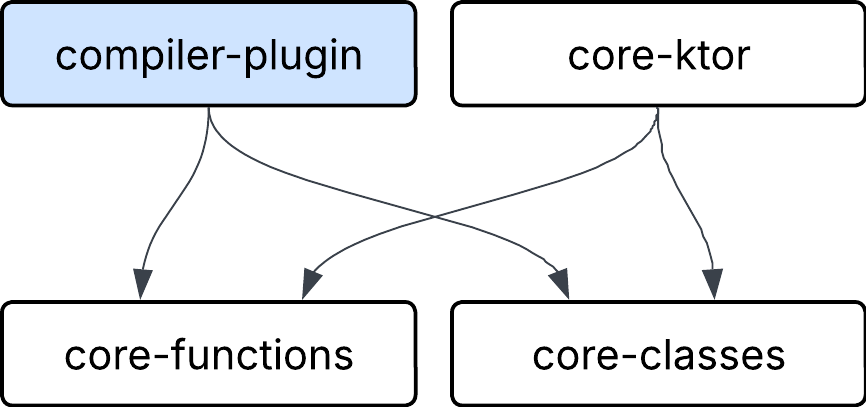
\includegraphics[width=.55\textwidth]{module-graph}
  \end{center}
  \caption{Module dependency graph}\label{module_dependency_graph}
\end{figure}

Now is a good time to take a look at architecture of kotlin-remote framework. At \ref{module_dependency_graph} is shown
module dependency graph of the framework. Each rectangle is a Gradle module. Before we only described
\ki{compiler-plugin} and \ki{core-functions} module. But there are two more modules that extend functionality of 
the mentioned ones. \ki{core-classes} contain support for distributed objects and \ki{core-ktor} provides an 
implememntation of the transport protocol for Kotlin Remote using Ktor.

\subsection{Ktor integration}
Kotlin Remote is meant to be transport agnostic. This is done by splitting code into three modules:
\kotlini{core-functions}, \ki{core-classes}, \ki{core-ktor}. Until now, we almost exclusively have
been discussing \ki{core-functions} module that contains logic related to remote functions. Now let us
briefly discuss \ki{core-ktor} module which contains Kotlin Remote integration with Ktor. Ktor is a
mature framework that offers lots of functions like auth support, logging etc. Kotlin Remote used
together with Ktor supports the same functionality Ktor does. For example, authentication can be
supported using code from listing \ref{auth_example}. Notice call to \ki{handleRemoteCall} function
in \ki{server}. This function passes control to \ki{core-ktor} module that deserializes arguments
of remote call, invokes remote function, serializes and sends result to the client. Inside
\ki{/call} route \ki{handleRemoteCall} is called implicitly.

\begin{listing}[!h]
  \begin{minted}{kotlin}
  val server = embeddedServer(Netty, port = 8080) {
    install(Authentication) {
      basic("auth-basic") { validate { ... } }
    }
    install(KRemote) { callableMap = genCallableMap() }
    routing {
      authenticate("auth-basic") {
        post("/callAuth") {
          println("Welcome to the protected route!")
          handleRemoteCall()
        }
      }
      remote("/call")
    }
  }

  data object AuthServerConfig : RemoteConfig {
    override val client: RemoteClient = HttpClient {
      ...
      install(Auth) { ... }
    }.remoteClient(genCallableMap(), "/callAuth")
  }
  \end{minted}
  \caption{Authentication support}\label{auth_example}
\end{listing}

\subsection{Remote classes}

Because Kotlin is not only procedural and functional language but also relies heavily on OOP, it
was decided to add support to call methods of the classes remotely, not only top-level functions.
Basic support for that is achieved easily. The only important difference between top level
functions and method function is that methods have implicit \ki{this} parameter. In our case we can
think about \ki{this} parameter just like about any other regular parameter. So calling a remote
method serializes \ki{this} and other method parameters on client, sends call on sever, server
deserializes \ki{this} and other parameters and calls method on deserialized \ki{this}. The good
news are this is already supported without any additional effort because Kotlin compiler treats
\ki{this} as a regular parameter of the function. But there are two huge problems with this
approach. Firstly, \ki{this} should be serializable, and serialization logic should be provided by
the user. Secondly, methods that mutate \ki{this} will mutate deserialized copy of \ki{this}, which
basically means that they will have no effect on the original \ki{this}. 

All these problems are not new and were addressed in lots of existing RMI frameworks, like Java RMI. 
In Kotlin Remote we decided to use well-known approach to solve these problems: stubs. Classes in 
Kotlin Remote can be marked with \ki{@RemoteSerializable} annotation. For each remote serializable class
custom \texttt{kotlinx.serialization} serializer is generated. 

This custom serializer serializes remote class as stub. Stub is a subclass of remote class that 
is generated for every remote class. Stub only has two fields: ID and URL of the machine it was created on. 
During serialization of remote class it is added to the special map called \ki{RemoteInstancesPool}. 
Keys in this pool are stub IDs and values are original classes. 

Stub is deserialized either as original class in case it is deserialized on the machine it was 
serialized on and \ki{RemoteInstancesPool} contains it, or as just stub. To understand whether stub 
was serialized on a certain machine, URL of this machine is compared with URL from the stub.

This URL is only used for this disambiguation of the nodes and garbage collection 
(more about it later in \ref{garbade_collection_section}). This URL is not used to make remote calls at all,
address of the target machine is still received from context parameter of remote functions. URL is specified
on the server when application is configured. It means that user should know address of the machine 
the server is running on.

Basically stubs are "remote references" that are supported by Kotlin Remote without altering logic
related to remote function. Only serialization functionality is changed. Because of that logic
related to remote classes lives in a separate Gradle module named \texttt{core-classes} which
neither depends nor is dependent on \texttt{core-functions} module described earlier. It is worth
noticing that stubs are serialized as is, this allows to pass remote references from one machine to
another even if reference is created on a third machine.

\subsubsection{Remote classes code generation}

It was said that for each \ki{@RemoteSerializable} class a stub subclass is generated. This
subclass is generated inside original class like on listing \ref{remote_class_stub}.
\ki{RemoteClassStub} extends \ki{Calculator} and implements interface \ki{Stub}. \ki{Stub}
interface can be used by user to check whether a certain instance of \ki{Calculator} a stub or not.
Notice how \ki{RemoteClassStub} invokes \ki{Calculator}'s default constructor even though
\ki{Calculator} doesn't have one. This is achieved by generating default constructor for
\ki{Calculator} in Kotlin Remote backend compiler plugin. \ki{Calculator} is also made open
implicitly by the same plugin on backend. Because these changes are made on backend,
\ki{Calculator} class cannot be extended, and its default constructor cannot be called from user
defined Kotlin code. Only code generated by compiler plugin can do that.

\begin{listing}[!h]
  \begin{minted}{kotlin}
  @RemoteSerializable
  class Calculator(private var init: Int) {
    @Remote
    context(_: RemoteContext<RemoteConfig>)
    suspend fun multiply(x: Int): Int {
        init *= x
        return init
    }
    class RemoteClassStub(
        override val id: Long,
        override val url: String
    ) : Calculator(), Stub
  }
  \end{minted}
  \caption{Remote class stub}\label{remote_class_stub}
\end{listing}

Unfortunately, without reflection (and we cannot use it because of KMP) it is unclear how to deserialize
\ki{Calculator} as its \ki{RemoteClassStub} because every remote class has its own \ki{RemoteClassStub} type.
To solve this issue another Kotlin Remote intrinsic is used, called \ki{genRemoteClassList}.
Take a look at listing \ref{gen_remote_class_list}. List of \ki{RemoteClassDescriptor} is used to generate
serializers and deserializers for remote classes using contextual serialization from \texttt{kotlinx.serialization}.

\begin{listing}[!h]
  \begin{minted}{kotlin}
  data class RemoteClassDescriptor<T : Any>(
    val clazz: KClass<T>,
    val serialName: String,
    val stubFabric: (Long, String) -> T,
  )

  fun genRemoteClassList(): List<RemoteClassDescriptor<Any>> = RemoteIntrinsic
  \end{minted}
  \caption{genRemoteClassList intrinsic}\label{gen_remote_class_list}
\end{listing}

\subsection{Garbage collection}\label{garbade_collection_section}

Now there is no way to remove remote classes from \ki{RemoteInstancesPool}. This is a serious
resource leak. To resolve this issue several techniques can be used, including reference counting
or full-blown distributed garbage collection. But we decided to opt for leasing approach, because
it is easy, lightweight and durable. Each time stub is deserialized on a machine this machine
begins sending lease requests to machine where original class of the stub is stored. To determine
address of the machine where original class is stored \ki{url} field of the stub is used. When
machine with original class does not get lease requests for specific class for a long time it
removes this class from \ki{RemoteInstancesPool}. Machine owning a stub stops sending lease
requests when this stub is garbage collected on the owner machine. To implement that weak
references are used. These are references that are not taken into account to mark reachable objects
during garbage collection. This is basically the whole algorithm. The beauty of this approach is
that when client owning a stub crashes, server is able to remove original class from its pool
gracefully. Garbage collection is enabled by default, but can be disabled and fine-tuned when needed. 
Ktor integration provides transport for leases, user can provide its own ways to deliver leases.

\section{Evaluation of the Kotlin Remote}

This section discusses criteria that are used to evaluate the
research results. Make sure your results can be used to published
research results, i.e., to the already known state-of-the-art.

(target size: 5-10 pages)

\subsection{Examples}

\subsection{Comparison to alternatives}

\subsubsection{gRPC}

\subsubsection{Kotlin RPC}

\section{Conclusions}

Summarize the main aspects and results of the research
project. Provide an answer to the research questions stated earlier.

(target size: 1/2 page)

\newpage
%\bibliographystyle{unsrt}
%\bibliography{msc-sample}
\printbibliography

\clearpage
\appendix
\section{Typesetting Examples}

\subsection{Code Fragments}

\begin{minted}{rust}
fn num_to_ordinal_expr(x: u32) -> String {
    format!("{}{}", x, match (x % 10, x % 100) {
        (1, 1) | (1, 21...91) => "st", 
        (2, 2) | (2, 22...92) => "nd", 
        (3, 3) | (3, 23...93) => "rd", 
        _ => "th" 
    }) 
} 
\end{minted}

\subsection{Tables}

\begin{table}[ht]
  \begin{center}
    \begin{tabular}{cl}
      \toprule
      Number & Description \\
      \midrule
      7 & A lucky number in Western culture \\
      8 & A lucky number in Chinese and other Asian cultures \\
      42 & Answer to the ultimate question of life, the universe, and everything \\
      404 & Not found \\
      \bottomrule
    \end{tabular}
    \caption{Useless insights I gained with no further meaning}
  \end{center}
\end{table}

\subsection{Plots}

\begin{figure}[ht]
  \begin{center}
    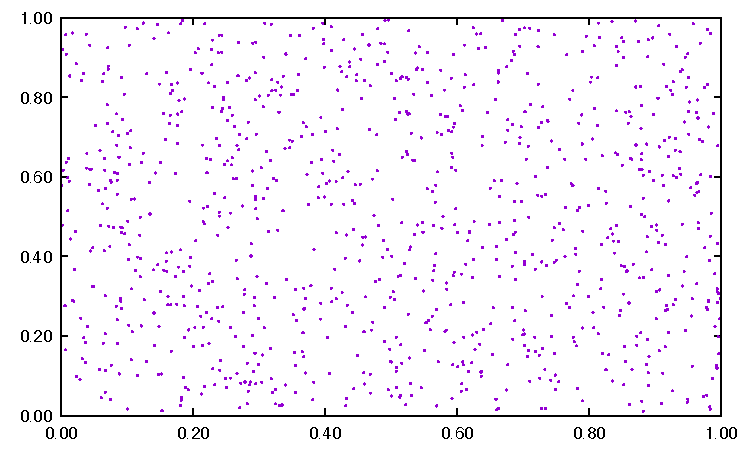
\includegraphics[width=.8\textwidth]{msc-plot}
  \end{center}
  \caption{Many dots distributed over a two dimensional unit space
    without any discernible pattern or deeper meaning}
\end{figure}

\end{document}
